\documentclass[a4paper,10pt]{article}

\usepackage[english]{babel}
\usepackage{graphicx}
\usepackage{rotating}
\usepackage{amsmath}

\usepackage{float} % for [H]
\usepackage[colorlinks, linkcolor=black, citecolor=black, urlcolor=black]{hyperref}
\usepackage{geometry}
\usepackage{svg}
%\usepackage{epstopdf}
%\epstopdfDeclareGraphicsRule{.svg}{pdf}{.pdf}{rsvg-convert -f pdf -o \OutputFile \InputFile}
\geometry{tmargin=3cm, bmargin=2.2cm, lmargin=2.2cm, rmargin=2cm}
\usepackage{todonotes} %Used for the figure placeholders
\usepackage{ifthen}
\usepackage{booktabs} %For better table formatting
\usepackage{longtable} %For tables that span multiple pages
\usepackage{array} %For column formatting
\usepackage{tabularx} %For flexible table column widths
\usepackage{tikz}
\usetikzlibrary{shapes, arrows.meta, positioning, fit, backgrounds, calc}
\usepackage{listings}
\usepackage{xcolor}

% Modern light code listing style for C
\definecolor{codebg}{RGB}{250,250,250}
\definecolor{codecomment}{RGB}{106,115,125}
\definecolor{codestring}{RGB}{80,161,79}
\definecolor{codekeyword}{RGB}{167,29,93}
\definecolor{codenumber}{RGB}{150,150,150}
\definecolor{codetext}{RGB}{36,41,46}
\definecolor{codeborder}{RGB}{225,228,232}

\lstdefinestyle{cstyle}{
    backgroundcolor=\color{codebg},
    commentstyle=\color{codecomment}\itshape,
    keywordstyle=\color{codekeyword},
    numberstyle=\tiny\color{codenumber},
    stringstyle=\color{codestring},
    basicstyle=\ttfamily\scriptsize\color{codetext},
    breakatwhitespace=false,
    breaklines=true,
    captionpos=b,
    keepspaces=true,
    numbers=none,
    showspaces=false,
    showstringspaces=false,
    showtabs=false,
    tabsize=4,
    frame=single,
    framerule=0.5pt,
    rulecolor=\color{codeborder},
    xleftmargin=1.5em,
    framexleftmargin=1em,
    framextopmargin=4pt,
    framexbottommargin=4pt,
    aboveskip=1em,
    belowskip=0.5em
}

\setlength{\parindent}{0pt}

% Your name and student number must be filled in on the title page found in
% titlepage.tex.

\begin{document}
\newboolean{anonymize}
% Uncomment to create an anonymized version of your report
%\setboolean{anonymize}{true}

\begin{titlepage}
    \newpage
    \thispagestyle{empty}
    \frenchspacing
    \hspace{-0.2cm}
    \includegraphics[height=3.4cm]{sedes}
    \hspace{0.2cm}
    \rule{0.5pt}{3.4cm}
    \hspace{0.2cm}
    \begin{minipage}[b]{8cm}
        \Large{Katholieke\newline Universiteit\newline Leuven}\smallskip\newline
        \large{}\smallskip\newline
        \textbf{Master of Engineering Science\newline Artificial Intelligence}\smallskip
    \end{minipage}
    \hspace{\stretch{1}}
    \vspace*{3.2cm}\vfill
    \begin{center}
        \begin{minipage}[t]{\textwidth}
            \begin{center}
                \LARGE{\rm{\textbf{\uppercase{Privacy Impact Assessment}}}}\\
                \Large{\rm{Macless-Haystack}}
            \end{center}
        \end{minipage}
    \end{center}
    \vfill
    \hfill\makebox[8.5cm][l]{%
        \vbox to 7cm{\vfill\noindent
            \ifthenelse{\boolean{anonymize}}{%
                {\rm \textbf{Anonymized}}\\
                {\rm Academic year 2025--2026}
            }{%
                {\rm \textbf{Lili De Bruyn (r0848166)}}\\
                {\rm \textbf{Annemerel Bobbaers (r0897155)}}\\
                {\rm \textbf{Magnus De Maerteleire (r0889456)}}\\
                {\rm \textbf{Jeff Jambé (r0902205)}}\\[2mm]
                {\rm Academic year 2025--2026}
            }
        }
    }
\end{titlepage}


\tableofcontents
\newpage

% Introduction/Executive Summary
\section{Introduction}
This report presents a Privacy Impact Assessment (PIA) for Macless-Haystack \cite{maclesshaystack}, an open-source (research) project that enables users to use Apple's 'Find My' network without requiring Apple hardware. As the technology for global tracking systems becomes increasingly more accessible by the introduction of global distributed networks such as the Apple 'Find My', Google 'Find My Device' and Amazon 'Sidewalk' networks, understanding the privacy implications of such technologies is important for both developers and users.
\bigskip

The report examines how Macless-Haystack collects, processes and stores data. It identifies potential privacy risks and proposes technical solutions to mitigate these concerns. We analyze the system from multiple perspectives: the tracker devices themselves, the Macless-Haystack application and API.
\bigskip

This report is structured in three main parts. First, we provide a detailed description of the application's functionality, stakeholders, and data collection practices. Second, we conduct a privacy impact assessment that includes a threat model, identification of privacy issues, and an analysis of specific threats. Finally, we present recommendations for addressing the identified privacy concerns, with particular focus on technical implementations that can be tested and verified.
\begin{figure}[H]
    \centering
    \begin{minipage}[t]{0.48\textwidth}
        \centering
        \includegraphics[width=\linewidth]{figures/application_screenshot.png}
        \caption{Screenshot of the Macless-Haystack application}
        \label{fig:screenshot}
    \end{minipage}
    \hfill
    \begin{minipage}[t]{0.48\textwidth}
        \centering
        \includegraphics[width=\linewidth]{figures/applicationoverview.png}
        \caption{High-level overview of the macless-haystack / Apple airtag application \cite{DBLP:journals/corr/abs-2103-02282}}
        \label{fig:macless-haystack}
    \end{minipage}
\end{figure}
% Part 1: Application Description (max 1500 words)
\section{Application Description}

\subsection{Functionality of the Application}
Macless-Haystack builds upon the OpenHaystack \cite{openhaystack} project, which reverse engineered the Apple 'Find My' application that enables the tracking of low cost Bluetooth devices without the need of an internet connection.
\bigskip

At a high level, the tracker broadcasts an identifier which can be detected by nearby Apple devices. These Apple devices then anonymously upload an encrypted report which contains it's current GPS location. The owner can later retrieve the location of their tracker by requesting these reports.
Figure~\ref{fig:macless-haystack} above visually represents the four main stages of the application:

\begin{enumerate}
    \item \textbf{Initial setup}: The process begins with the owner pairing their device, this means generating a unique private and public (advertisement) key pair and programming the advertisement key onto the tracker.
    \item \textbf{Broadcast}: After setup, the tracker begins broadcasting Bluetooth packets that are based on its advertisement key. Apple devices nearby act as a finder device and can pick up on these advertisements.
    \item \textbf{Upload encrypted location reports}: When a finder device detects an advertisement, it generates a report containing its current GPS location. This location is then encrypted using the advertisement key broadcasted by the device, making it inaccessible to everyone except the owner. The encrypted report is uploaded to Apple's servers.
    \item \textbf{Download and decrypt location reports}: Anyone with access to the key-pair can then request the location reports linked to the tracker's keys. Using the matching private key, the owner can decrypt these reports get the trackers location.
\end{enumerate}

\begin{figure}[ht]
    \centering
    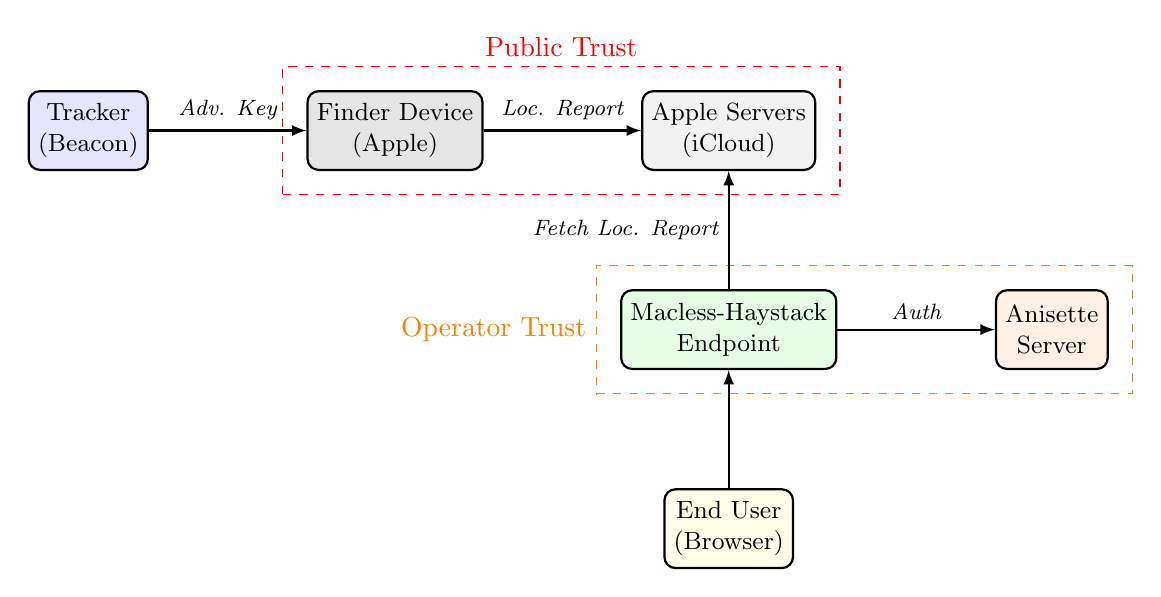
\begin{tikzpicture}[
        node distance=1.5cm and 2cm,
        entity/.style={rectangle, draw=black, thick, fill=white, rounded corners, minimum height=1cm, align=center, font=\small},
        boundary/.style={dashed, red, thick},
        link/.style={->, >=latex, thick},
        labeltext/.style={font=\footnotesize\itshape}
    ]

    % Nodes
    \node[entity, fill=blue!10] (tracker) {Tracker\\(Beacon)};
    \node[entity, right=of tracker, fill=gray!20] (finder) {Finder Device\\(Apple)};
    \node[entity, right=of finder, fill=gray!10] (apple) {Apple Servers\\(iCloud)};
    
    \node[entity, below=of apple, fill=green!10] (endpoint) {Macless-Haystack\\Endpoint};
    \node[entity, right=of endpoint, fill=orange!10] (anisette) {Anisette\\Server};
    
    \node[entity, below=of endpoint, fill=yellow!10] (user) {End User\\(Browser)};

    % Edges
    \draw[link] (tracker) -- node[above, labeltext] {Adv. Key} (finder);
    \draw[link] (finder) -- node[above, labeltext] {Loc. Report} (apple);
    \draw[link] (endpoint) -- node[left, labeltext] {Fetch Loc. Report} (apple);
    \draw[link] (endpoint) -- node[above, labeltext] {Auth} (anisette);
    \draw[link] (user) -- node[right, labeltext] {} (endpoint);

    % Trust Boundaries
    
    % Public Trust (Tracker Output + Apple Infrastructure)
    \begin{scope}[on background layer]
        \node[fit=(finder)(apple), draw=red, dashed, inner sep=0.3cm, label={[red]above:Public Trust}] {};
    \end{scope}

    % Operator Trust
    \begin{scope}[on background layer]
        \node[fit=(endpoint)(anisette), draw=orange, dashed, inner sep=0.3cm, label={[orange]left:Operator Trust}] {};
    \end{scope}

    \end{tikzpicture}
    \caption{Stakeholders and Trust Boundaries Diagram}
    \label{fig:stakeholders}
\end{figure}
\subsection{The Stakeholders}
The primary stakeholders are the end users who want to research the 'Find My' network and track their own Bluetooth devices.
They are responsible for generating the keypairs used in the system and storing them safely, as well as programming the advertisement key onto the tracker.

\bigskip
The Macless-Haystack API operator is the party running the backend that accesses the 'Find My' network and fetches encrypted location reports. In practices this is the same party as the end user because to our knowledge no public Macless-Haystack API endpoints exist.

\bigskip
The Anisette server operator runs the separate service that Macless-Haystack API connects to in order to emulate a real Apple device during login and communication with Apple. This role can again coincide with the endpoint operator in a self-hosted setup, but when a public or third-party Anisette instance is used, that operator becomes a distinct stakeholder who may see sensitive authentication-related traffic and must therefore be explicitly trusted.

\bigskip
Apple is an indirect but essential stakeholder, as it's 'Find My' and iCloud infrastructure receive the encrypted location reports from nearby Apple devices and serves them to the Macless-Haystack endpoint.
To further visualise the stakeholders and their relationships, see Figure~\ref{fig:stakeholders}.
\bigskip

In essence, the only sensitive data in the system is the private key of the tracker. The encrypted location reports and the advertisement key are public information as anyone that is physically close to the tracker can read the advertisement key and request the encrypted location reports.
This means that all data that flows through this part of the system is public information, and should contain no (accessible) personal data. An important detail that is not in the diagram is that the finder device itself generates and encrypts the location reports, this internal data is very personal and is defintely not public information. 

\bigskip
The data in the operator endpoint, however, could contain some personal data, depending on the hosting setup.
Conventionally, the endpoint operator only has access to metadata and the encrypted location reports, which are public information.
If the endpoint operator requests the Apple ID and password of the end user, and uses this to login to Apple and fetch the encrypted location reports.
Additional trust must be had in it as these credentials could be used for non 'Find My' purposes.

\bigskip


\subsection{Types of Data Collected and Purposes}
The system involves multiple components, each collecting different types of data. Table~\ref{tab:data_collection_summary} provides an overview of data collection across the entire Macless-Haystack ecosystem.

\begin{table}[H]
    \centering
    \caption{Summary of Data Collection across System Components}
    \label{tab:data_collection_summary}
    \begin{tabularx}{\textwidth}{@{}l X X@{}}
        \toprule
        \textbf{Component} & \textbf{Data Collected \& Stored} & \textbf{Purpose \& Privacy Implications} \\
        \midrule
        \textbf{Tracker} & None (Broadcasts Public Key) & Operates solely to broadcast the advertisement key. \\
        \addlinespace
        \textbf{Finder Device} & Advertisement Key, GPS Location, Signal Strength, Time. & Detects trackers. Data is typically deleted from the device after $\approx$5 mins unless in airplane mode. \\
        \addlinespace
        \textbf{Apple Servers} & Advertisement Key, Encrypted Location Report. & Central storage. Allows querying of location reports. \\
        \addlinespace
        \textbf{Macless App} & Private Keys, Auth Credentials. & Viewing tracker location (history). \\
        \addlinespace
        \textbf{Macless API} & Request Logs (Advertisement Keys), API Requests. & API logging reveals which keys are being tracked. \\
        \bottomrule
    \end{tabularx}
\end{table}

\subsubsection{Data Collection Details in Apple's Ecosystem}
Since Apple's implementation is closed-source, we rely on community reverse-engineering efforts to understand the data collection process. A blog post analyzing the finder device~\cite{binaryhick2025searchparty} discovered that when an Apple device detects a tracker, it temporarily stores the advertisement key, GPS location, Bluetooth signal strength (RSSI), timestamp, and other metadata.
This data is reportedly deleted quickly (within ~5 minutes), though users can extend this by enabling airplane mode. Apple also employs algorithms to detect unwanted tracking, which may trigger additional data retention on the finding device.
Once uploaded, Apple stores the advertisement key and the encrypted location report. While the location report itself is encrypted, the metadata, such as the uploader's IP address could be visible to Apple.
This creates a theoretical risk where Apple could link a tracker to a specific user if that user's own (Apple) devices frequently reports the tracker's location. Furthermore, Apple could identify Macless-Haystack operators and potentially terminate the associated Apple IDs to prevent abuse however this has not been reported to happen in practice.
% Part 2: Privacy Impact Assessment (max 2500 words)
\section{Privacy Impact Assessment}

\subsection{Threat Model}
The system's privacy properties depend on several trust assumptions. Users must trust Apple's infrastructure to provide end-to-end encryption (though Apple could have metadata visibility) and the endpoint operator to protect stored credentials and logs. The primary trust boundaries exist at: (1) Bluetooth broadcasts between the tracker and nearby devices, (2) network communication between the frontend and backend, (3) authenticated connections to Apple's servers, and (4) filesystem access on the server. These boundaries represent the main points where information can be compromised, as detailed in the threat analysis below.    

\subsection{LINDDUN Privacy Threat Analysis}
Using the detailed dataflow diagram (Figure~\ref{fig:dataflow_diagram}) and the LINDDUN framework, we can analyze the privacy threats in the system.
As the current diagram is very small, a large full page version is included in the Appendices \ref{fig:dataflow_diagram_full}.
\begin{figure}[H]
    \centering
    \includegraphics[width=\textwidth]{figures/dataflow.png}
    \caption{Dataflow Diagram of the Macless-Haystack System}
    \label{fig:dataflow_diagram}
\end{figure}

\begin{longtable}{|>{\raggedright\arraybackslash}p{1.3cm}|>{\raggedright\arraybackslash}p{2.2cm}|>{\raggedright\arraybackslash}p{3.8cm}|>{\raggedright\arraybackslash}p{1.8cm}|>{\raggedright\arraybackslash}p{1.3cm}|>{\raggedright\arraybackslash}p{3.8cm}|}
\caption{LINDDUN Privacy Threat Analysis}\label{tab:lindunn}\\
\hline
\textbf{Code} & \textbf{Threat Category} & \textbf{Description} & \textbf{Affected Interaction(s)} & \textbf{Severity} & \textbf{Mitigation} \\
\hline
\endfirsthead
\hline
\textbf{Code} & \textbf{Threat Category} & \textbf{Description} & \textbf{Affected Interaction(s)} & \textbf{Severity} & \textbf{Mitigation} \\
\hline
\endhead
\hline
\endfoot
NC.3 / II.1 & Non-Compliance & Apple ID and password can be stored in plain text in config.ini (optional but supported). Exposes credentials to anyone with filesystem access (to the Macless-Haystack server).  & Interaction 8 & Critical & Remove plain text password storage\\
\hline
DD.4.2 / NC.2 & Data Disclosure / Non-Compliance & Storage of private and public keys in plain text. Keys should be stored using platform-specific secure storage (Apple Keychain, Android Keystore, GNOME Keyring, Windows Credential Manager). & Interaction 2, 3b & High & Implement secure key storage using platform APIs (e.g., flutter\_secure\_storage) \\
\hline
L.1.1 / I.2.2.b & Linkability / Information Disclosure & Static advertisement keys allow tracking of device presence. The system broadcasts the same public key continuously, enabling anyone to determine if the tracked device is nearby. & Interaction 4 & High & Implement rolling keys. \\
\hline
NC.3.c & Non-Compliance & Weak authentication: no authentication required by default, or single username/password shared among all users of an endpoint instance. & Interaction 16, 24 & High & Implement per-user authentication (e.g., OAuth) \\
\hline
U.1.2 & Unawareness & Users are not informed that sharing their private key with others enables complete location tracking of their device. Lacks clear privacy warnings. & Interaction 2 & Medium & Add privacy warnings in documentation, UI when exporting keys \\
\hline
NC.1.2.a & Regulatory Non-Compliance & Violation of Apple's EULA by creating custom AirTag-like devices using Apple's 'Find My' network infrastructure. & Interaction 3a, 4 & Medium & Add legal disclaimer; make users assume responsibility \\
\hline
D.3 & Detectability & Static advertisement keys allow querying Apple servers to determine if a tracker is still active by checking for new location reports, even without decryption. & Interaction 4, 20 & Medium & rolling keys solves this.  \\
\hline
NR.1.1.a & Non-Repudiation & Apple ID is attached to all location report requests, allowing Apple to identify and track Macless-Haystack server hosters and their query patterns. & Interaction 20,13 & Medium & Inherent to Apple's authentication, no solution without protocol changes \\
\hline
NC.1.2.b & Regulatory Non-Compliance & Reverse engineering and accessing iCloud authentication from non-Apple devices violates Apple's EULA & Interaction 20,13 & Medium & Legal disclaimer; users assume legal responsibility \\
\hline
L.2.2.1 & Linkability & Sending advertisement keys to potentially public endpoint links user's IP address with their tracked devices. & Interaction 16, 24 & Medium & Only use trusted, self-hosted endpoints \\
\hline
NC.3.b & Non-Compliance & HTTP access is supported (non-mandatory HTTPS), exposing advertisement keys during transmission. & Interaction 16,24 & Medium & Enforce HTTPS\\
\hline
I.1.2 & Information Disclosure & Apple servers receive query metadata revealing usage patterns. & Interaction 20, 23 & Low & Inherent to protocol; making fake queries to obfuscate real usage patterns\\
\hline
\end{longtable}
\newpage
\subsection{Main Identified Privacy Threats}
\subsubsection{Plain Text Credentials}
The current implementation stores authentication tokens and passwords in plain text files that can be read directly without decryption\footnote{Remote shell access is a common objective for attackers, such as the critical flaw recently discovered in the React library. Consequently, the file system cannot be trusted simply because the enduser can't directly access it.}. The auth.json file contains authentication tokens (dsid and searchPartyToken) used to communicate with Apple's servers instead of passwords after initial login. These tokens are stored as plain text JSON, meaning anyone with file system access can read them directly. Similarly, passwords in config.ini are stored in plain text, allowing direct reading of sensitive credentials. In the code snippet below, you can see how we test for plain text credentials.
Config.ini is not written to by the program resulting in it not being able to be unit tested in the traditional sense. To ensure privacy, we added a specific test to read the file and check that it does not contain any plain text passwords.
\begin{lstlisting}[style=cstyle, language=Python, caption={Test showing plain text credential storage}, label={lst:credential_test}, basicstyle=\ttfamily\tiny\color{codetext}]
class TestCredentialStorage:
    def test_config_does_not_store_plaintext_passwords(self):
        config_path = mh_config.getConfigPath() + "/config.ini"
            
        has_plaintext = False
        with open(config_path, 'r') as f:
            for line in f:
                for field in ['appleid_pass', 'endpoint_pass']:
                    match = re.match(rf'{field}\s*=\s*(.*)$', line.strip())
                    if match:
                        has_plaintext = True
        assert not has_plaintext, "config.ini contains plaintext passwords"

    @mock.patch("endpoint.mh_endpoint.pypush_gsa_icloud.icloud_login_mobileme")
    @mock.patch("endpoint.mh_config.getConfigFile", return_value="test.json")
    @mock.patch("endpoint.mh_endpoint.json.dump")
    @mock.patch("endpoint.mh_endpoint.open", new_callable=mock.mock_open)
    def test_auth_json_does_not_include_sensitive_fields(self, mock_file, mock_json_dump, mock_get_config, mock_icloud_login):
        fake_mobileme = StrDict("MobileMe Result")
        fake_mobileme.d = {
            'dsid': 'FAKE_DSID',
            'delegates': {
                'com.apple.mobileme': {
                    'service-data': {
                        'tokens': {'searchPartyToken': 'FAKE_TOKEN'}
                    }
                }
            }
        }
        mock_icloud_login.return_value = fake_mobileme

        mh_config.USER = "fakeuser"
        mh_config.PASS = "fakepass"
        
        mh_endpoint.getAuth(regenerate=True)

        
        args, _ = mock_json_dump.call_args
        data = args[0]
        
        assert 'searchPartyToken' not in data, "searchPartyToken should not be stored in auth.json"
        assert 'dsid' not in data, "dsid should not be stored in auth.json"

    # The key generation script's procedural style makes standard unit testing not possible.
    # We tested it by mocking the environment and executing the script string directly.
    @mock.patch('shutil.rmtree')
    @mock.patch('os.path.exists', return_value=False)
    @mock.patch('os.mkdir')
    @mock.patch('builtins.open')
    def test_private_key_not_stored_as_plain_text(self, mock_open, mock_mkdir, mock_exists, mock_rmtree):
        file_mocks = {}
        def open_side_effect(filename, mode='r', *args, **kwargs):
            m = mock.MagicMock()
            m.__enter__.return_value = m
            file_mocks[filename] = m
            return m
        mock_open.side_effect = open_side_effect

        # Execute script
        with mock.patch.object(sys, 'argv', ["generate_keys.py", "-n", "1", "--prefix", "TEST"]):
            exec(generate_keys, {})

        target_path = 'output/TEST_devices.json'
        if target_path not in file_mocks:
            pytest.fail(f"Devices file {target_path} was not opened. Captured: {list(file_mocks.keys())}")

        target_file = file_mocks[target_path]
        
        full_content = ""
        for call in target_file.write.mock_calls:
            if call.args:
                full_content += call.args[0]
                
        device_data = json.loads(full_content)        
        
        for device in device_data:
            if device.get('privateKey'):
                pytest.fail(f"Private key found in plain text")
\end{lstlisting}
\bigskip
\begin{lstlisting}[style=cstyle, caption={Test Output showing privacy failures}, label={lst:credential_test_output}, basicstyle=\ttfamily\tiny\color{codetext}, keywords={FAILED, AssertionError, Failed}, keywordstyle=\color{red}\bfseries, moredelim={[l][\color{red}]{E\ \ }}]
========================= test session starts =========================
platform linux -- Python 3.10.19, pytest-8.4.2, pluggy-1.6.0 -- /home/cyuzuzo/.pyenv/versions/3.10.19/bin/python3.10
cachedir: .pytest_cache
rootdir: /home/cyuzuzo/Projects/macless-haystack
configfile: pytest.ini
plugins: anyio-4.11.0
collected 3 items                                                                                                                                                                                        

test_security_pytest.py::TestCredentialStorage::test_config_does_not_store_plaintext_passwords FAILED
test_security_pytest.py::TestCredentialStorage::test_auth_json_does_not_include_sensitive_fields FAILED
test_security_pytest.py::TestCredentialStorage::test_private_key_not_stored_as_plain_text FAILED                   

========================= FAILURES =========================
_____ TestCredentialStorage.test_config_does_not_store_plaintext_passwords _____
test_security_pytest.py:60: in test_config_does_not_store_plaintext_passwords
    assert not has_plaintext, "config.ini contains plaintext passwords"
E   AssertionError: config.ini contains plaintext passwords
E   assert not True
_____ TestCredentialStorage.test_auth_json_does_not_include_sensitive_fields _____
test_security_pytest.py:98: in test_auth_json_does_not_include_sensitive_fields
    assert 'searchPartyToken' not in data, "searchPartyToken should not be stored in auth.json"
E   AssertionError: searchPartyToken should not be stored in auth.json
E   assert 'searchPartyToken' not in {'dsid': 'FAKE_DSID', 'searchPartyToken': 'FAKE_TOKEN'}
_____ TestCredentialStorage.test_private_key_not_stored_as_plain_text _____
test_security_pytest.py:139: in test_private_key_not_stored_as_plain_text
    pytest.fail(f"Private key found in plain text")
E   Failed: Private key found in plain text
\end{lstlisting}
 \subsubsection{HTTP Communication}
The current Macless Haystack server implementation allows the endpoint to run over unencrypted HTTP when TLS certificates are not configured. The code checks for the presence of certificate files and falls back to HTTP if they are missing. This creates a security risk because all communication between client and server occurs in plain text, making it vulnerable to network sniffing and man-in-the-middle attacks. An attacker on the same network can intercept and read all traffic, including Basic Authentication credentials between the endpoint and the client that are only Base64-encoded and easily decoded.
\\
\begin{minipage}[t]{0.49\linewidth}
\begin{lstlisting}[style=cstyle, language=Python, caption={Test if http is allowed}, label={lst:https_test}, basicstyle=\ttfamily\tiny\color{codetext}]
class TestHTTPSConfiguration:
    @mock.patch("mh_endpoint.HTTPServer")
    @mock.patch("mh_endpoint.check_if_anisette_is_reachable")
    @mock.patch("os.path.isfile")
    def test_runs_without_certificate(self, mock_isfile, mock_check_anisette, mock_server):
        cert_path = mh_config.getCertFile()

        # mock the certificate file not existing
        def isfile_side_effect(path):
            if path == cert_path:
                return False
            return True
        mock_isfile.side_effect = isfile_side_effect
        
        mh_endpoint.main()
        
        mock_isfile.assert_any_call(cert_path)
        
        mock_server.return_value.serve_forever.assert_not_called()
\end{lstlisting}
\end{minipage}
\hfill
\begin{minipage}[t]{0.49\linewidth}
\begin{lstlisting}[style=cstyle, caption={Test output showing http is allowed}, label={lst:https_test_output}, basicstyle=\ttfamily\tiny\color{codetext}, keywords={FAILED, AssertionError, Failed}, keywordstyle=\color{red}\bfseries, moredelim={[l][\color{red}]{E\ \ }}]
===================== test session starts =====================
platform linux -- Python 3.10.19, pytest-8.4.2, pluggy-1.6.0 -- /home/cyuzuzo/.pyenv/versions/3.10.19/bin/python3.10
cachedir: .pytest_cache
rootdir: /home/cyuzuzo/Projects/macless-haystack
configfile: pytest.ini
plugins: anyio-4.11.0
collected 1 item                                                                                                                                                                                        

test_security_pytest.py::TestHTTPSConfiguration::test_runs_without_certificate FAILED

===================== FAILURES =====================
_____ TestHTTPSConfiguration.test_runs_without_certificate _____
test_security_pytest.py:49: in test_runs_without_certificate
    mock_http_server.return_value.serve_forever.assert_not_called()
../../.pyenv/versions/3.10.19/lib/python3.10/unittest/mock.py:890: in assert_not_called
    raise AssertionError(msg)
E   AssertionError: Expected 'serve_forever' to not have been called. Called 1 times.
E   Calls: [call()].
\end{lstlisting}
\end{minipage}   

%\todo[inline]{Add unit test for plain text credentials}

\subsubsection{Advertisement Keys in Macless Haystack}
In the current setup, each tracker continuously broadcasts a beacon containing the same static\footnote{The firmware supports the use of multiple static keys; This creates the exact same issue but to exploit it, you would need to observe the device over a longer period of time.} advertisement key. Any Apple device that receives such a packet takes its own location and encrypts that, so that only the trackers matching private key can decrypt it. Using a static public key introduces a serious linkability privacy problem. Because the same identifier is broadcasted in every packet, any nearby device with a simple BLE sniffer can record this constant over time, and across different places and then correlate all sightings as belonging to the same physical tracker. This means that anyone could build a detailed movement profile of the tagged object or person just by re-observing the same static key at different locations. The encryption protects the content of each report from being read but it does nothing to stop third parties from recognizing that this is the same beacon as yesterday and inferring sensitive patterns (home, workplace, daily routines) purely from repeated observations.
\\
\\
Additionally, if Apple is considered an untrustworthy entity, they could analyze the metadata accompanying location reports, such as the static advertisement key and the finding device's IP address to infer the user's approximate location and reconstruct movement patterns or daily routines.
\\
\\
A testing environment and test suite were developed to evaluate this behavior in the trackers firmware. To determine if static keys are being utilized, the \texttt{run\_openhaystack} function is called repeatedly while a shim replaces the Bluetooth advertising routine, enabling direct inspection of the broadcast payloads. Static codes are detected if multiple calls to \texttt{run\_openhaystack} trigger the BLE controller with identical payloads.
\\
\begin{minipage}[t]{0.48\linewidth}
\begin{lstlisting}[style=cstyle, language=C, caption={Unit Test used to check if static codes are being used}, basicstyle=\ttfamily\tiny\color{codetext}]
/**
 * @brief Test that multiple openhaystack_run calls use the same advertisement data
 * This proves non-rolling behavior by showing that
 * esp_ble_gap_config_adv_data_raw is called with identical data across multiple runs. 
 */
TEST(openhaystack_integration, multiple_runs_same_adv_data_within_cycle)
{
    TEST_ASSERT_EQUAL(0, openhaystack_init());

    uint8_t first_call_adv_data[31];

    const uint8_t TEST_REUSE_CYCLES = 5;
    const uint8_t TEST_DELAY_S = 1;

    for (int i = 0; i <= TEST_REUSE_CYCLES + 1; i++) {
        openhaystack_run(TEST_DELAY_S, TEST_REUSE_CYCLES);

        // On first iteration, store data
        if (i == 0) {
            memcpy(first_call_adv_data, last_adv_data, last_adv_data_len);

        } else if (i <= TEST_REUSE_CYCLES) {
            // Runs 1..TEST_REUSE_CYCLES should match Run 0
            TEST_ASSERT_EQUAL_UINT8_ARRAY_MESSAGE(
                first_call_adv_data,
                last_adv_data,
                last_adv_data_len,
                "Advertisement data should match during reuse window"
            );
        } else {
            // i == TEST_REUSE_CYCLES + 1 -> Should have rolled.
            TEST_ASSERT_NOT_EQUAL(0, memcmp(first_call_adv_data, last_adv_data, last_adv_data_len));
        }
    }
}
    \end{lstlisting}
    \end{minipage}
    \hfill
    \begin{minipage}[t]{0.48\linewidth}
    \begin{lstlisting}[style=cstyle, caption={Unit Test Output illustrating static key usage}, basicstyle=\ttfamily\tiny\color{codetext}]
Unity test run 1 of 1
Macless Haystack Test - Non-Rolling Code Privacy Test Suite
=============================================================

TEST(openhaystack_integration, multiple_runs_same_adv_data_within_cycle)I (604) BTDM_INIT: BT controller compile version [0f0c5a2]
I (604) BTDM_INIT: Bluetooth MAC: 0c:b8:15:f6:6c:fe
I (614) phy_init: phy_version 4791,2c4672b,Dec 20 2023,16:06:06
I (1044) macless_haystack: OpenHaystack Initializing in STATIC mode
E (1044) macless_haystack: Found 1 keys
I (1044) macless_haystack: OpenHaystack initialized with 1 keys
I (1054) macless_haystack: Loading key with index 0 at address 1
I (1054) macless_haystack: using key with start 93 44
I (1064) macless_haystack: Sending beacon
I (1174) macless_haystack: Current cycle is 0. Reusing key. 
I (1274) macless_haystack: Going to sleep
./main/main.c:119::FAIL: Expected Not-Equal

-----------------------
1 Tests 1 Failures 0 Ignored 
FAIL
\end{lstlisting}
\end{minipage}



\subsubsection{GDPR Compliance}
To assess GDPR compliance, we analyze the system based on the data controllers involved, the personal data they process.
\begin{longtable}{|>{\raggedright\arraybackslash}p{2.5cm}|>{\raggedright\arraybackslash}p{5cm}|>{\raggedright\arraybackslash}p{7cm}|}
\caption{GDPR Compliance Analysis by Data Controller}\label{tab:gdpr_stakeholders}\\
\hline
\textbf{Data controller} & \textbf{Personal Data Processed} & \textbf{GDPR Risks \& Violations} \\ \hline
\endfirsthead
\hline
\textbf{Data controller} & \textbf{Personal Data Processed} & \textbf{GDPR Risks \& Violations} \\ \hline
\endhead
\hline
\endfoot
\textbf{The End User} & Private keys, tracked objects. & 
\textbf{Integrity (Art 5, 32):} Insecure key storage (plain text JSON). \newline
\textbf{Lawfulness (Art 6):} Can more easily circumvents anti-stalking protections making non-consensual surveillance possible.\newline \textit{Household Exemption: Generally, for purely personal/household activities, GDPR may not apply (Art 2(2)(c)).} \\ \hline
\textbf{Endpoint Operator} & endpoint operators: Apple ID, Password\newline users meta data: Encrypted reports, timestamps, debug logs (with Advertisement Keys). & 
\textbf{Integrity \& Confidentiality:} unencrypted HTTP traffic (only applies if the data becomes linkable to a specific person), plain text credentials.\newline
\textbf{Transparency:} End user often uninformed about data processing; no documented purpose specification. \\ \hline
\textbf{Apple} & Encrypted location reports, advertisement keys & 
\textbf{Linkability:} In self-hosted setups, Apple could link the tracker to the owner's Apple ID.\newline
\textbf{Solution:} Rolling keys significantly reduce the ability to link reports to a person. \\ \hline
\end{longtable}

% Part 3: Recommendations (no specific word limit mentioned, but part of 4000 word total)
\section{Recommendations}
\subsection{Credential Encryption}
The backend of the application is written in python, so an appropriate way to store the secrets is using the "keyring" library. This library interacts with the OS level keychains, and provides a simple interface to store and retrieve credentials safely.
The following code snippets show how this can be implemented, in both cases a json load / plain text read has been replaced by a keyring.get\_password call.

\begin{minipage}[t]{0.48\linewidth}
\begin{lstlisting}[style=cstyle, language=Python, caption={Secure implementation for Apple ID retrieval}, label={lst:secure_config}, basicstyle=\ttfamily\tiny\color{codetext}]
def getUser():
    user = keyring.get_password("macless-haystack", "apple_id")
    if user:
        return user
    logger.error("Apple ID not found in keyring")
    return None

def getPass():
    username = getUser()
    if username:
        password = keyring.get_password("macless-haystack-appleid", username)
        if password:
            return password
    logger.error("Apple ID password not found in keyring")
    return None
\end{lstlisting}
\end{minipage}
\hfill
\begin{minipage}[t]{0.48\linewidth}
\begin{lstlisting}[style=cstyle, language=Python, caption={Secure implementation for authentication token storage}, label={lst:secure_auth}, basicstyle=\ttfamily\tiny\color{codetext}]
def getAuth(regenerate=False):
    service_id = "macless-haystack"
    username = "auth"
    stored_auth = keyring.get_password(service_id, username)

    if stored_auth and not regenerate:
        j = json.loads(stored_auth)
    else:
        logger.info('Trying to login')
        mobileme = icloud_login_mobileme(
            username=mh_config.getUser(), password=mh_config.getPass())

        logger.debug('Answer from icloud login')
        logger.debug(mobileme)
        status = mobileme['delegates']['com.apple.mobileme']['status']
        if status == 0:
            j = {'dsid': mobileme['dsid'], 'searchPartyToken': mobileme['delegates']
                 ['com.apple.mobileme']['service-data']['tokens']['searchPartyToken']}
            keyring.set_password(service_id, username, json.dumps(j))
        else:
            msg = mobileme['delegates']['com.apple.mobileme']['status-message']
            logger.error('Invalid status: ' + str(status))
            logger.error('Error message: ' + msg)
            if 'blocking' in msg:
                logger.error(
                    'It seems your account score is not high enough. Log in to https://appleid.apple.com/ and add your credit card (nothing will be charged) or additional data to increase it.')
            logger.error('Unable to proceed, program will be terminated.')

            sys.exit()
    return (j['dsid'], j['searchPartyToken'])
\end{lstlisting}
\end{minipage}
To solve the issue that the private-public key pairs are stored in plain text, a similar approach can be used using the flutter secure storage library.
This will require a reworking of the generate\_keys.py script as its currently written in python. The reason as to which it is better to port it into flutter is that sharing credentials saved in secure storage is non trivial and porting the short key generation script to flutter should be a small task.
\subsection{HTTPS Enforcement}
The server should enforce HTTPS and not allow HTTP fallback when TLS certificates are missing when deployed. Currently, the server falls back to unencrypted HTTP if certificate files are not found. The server startup should check for both the TLS certificate and private key files, and terminate with a clear error message if either is missing, rather than falling back to HTTP. For development and testing, a helper script should be provided to generate self-signed certificates, but production deployments should use certificates from a trusted certificate authority.
A small assertion can be added to the server to check if the certificate is there, if not, the server should exit with an error message. This prevents the server from running without a certificate.
\newpage
\begin{lstlisting}[style=cstyle, language=Python, caption={HTTPS Enforcement Logic}, basicstyle=\ttfamily\tiny\color{codetext}]
if os.path.isfile(mh_config.getCertFile()):
    logger.info("Certificate file " + mh_config.getCertFile() +
                " exists, so using SSL")
    ssl_context = ssl.SSLContext(ssl.PROTOCOL_TLS_SERVER)
    ssl_context.load_cert_chain(certfile=mh_config.getCertFile(
    ), keyfile=mh_config.getKeyFile() if os.path.isfile(mh_config.getKeyFile()) else None)

    httpd.socket = ssl_context.wrap_socket(httpd.socket, server_side=True)

    logger.info("serving at " + address + " over HTTPS")
else:
    logger.info("Certificate file not found, please provide a valid certificate file")
    logger.error("Exiting program")
    return
\end{lstlisting}

The following test output confirms that the recommendations solve the identified issues, with the exception of the private key storage which requires a more extensive changes as discussed.

\begin{lstlisting}[style=cstyle, caption={Final Security Test Results}, label={lst:final_security_test}, basicstyle=\ttfamily\tiny\color{codetext}, keywords={FAILED}, keywordstyle=\color{red}\bfseries, emph={PASSED}, emphstyle=\color{green}\bfseries]
===================== test session starts =====================
platform linux -- Python 3.10.19, pytest-8.4.2, pluggy-1.6.0 -- /home/cyuzuzo/.pyenv/versions/3.10.19/bin/python3.10
cachedir: .pytest_cache
rootdir: /home/cyuzuzo/Projects/macless-haystack
configfile: pytest.ini
plugins: anyio-4.11.0
collected 4 items

test_security_pytest.py::TestHTTPSConfiguration::test_runs_without_certificate PASSED [ 25%]
test_security_pytest.py::TestCredentialStorage::test_config_does_not_store_plaintext_passwords PASSED [ 50%]
test_security_pytest.py::TestCredentialStorage::test_auth_stored_securely_in_keyring PASSED [ 75%]
test_security_pytest.py::TestCredentialStorage::test_private_key_not_stored_as_plain_text FAILED [100%]
\end{lstlisting}

\subsection{Handling the GDPR and EULA Violations}
Our recommended solution to the GDPR and EULA violations is to obtain explicit consent from the user regarding the use of the application and the collection of their data. Additionally, it is important to inform users that the application is used at their own risk, and that they are advised to host the Macless-Haystack server themselves while being fully aware of the privacy implications associated with this application.

A similar disclaimer is included in the GitHub README.This information should be incorporated directly into the application itself, together with a clear consent form.

\subsection{Mitigating Linkability with Rolling Codes}
Static advertisement keys allow anyone to track a device by listening for its BLE signal. To fix this, we recommend using rolling codes, which means the key changes periodically (for example, every 24 hours).\\
To prevent this we can use the same method as Apple's official airtags \cite{DBLP:journals/corr/abs-2103-02282}. This uses Elliptic Curve Cryptography on the NIST P-224 curve. It starts with a master key pair and a 32-bit symmetric key. New keys are created using the ANSI X.963 key derivation function (KDF) with these formulas \cite{DBLP:journals/corr/abs-2103-02282}:
\begin{align}
SK_i &= \text{KDF}(SK_{i-1}, \text{``update''}, 32) \\
(u_i, v_i) &= \text{KDF}(SK_i, \text{``diversify''}, 72) \\
d_i &= (d_0 * u_i) + v_i \\
p_i &= d_i * G
\end{align}

This requires a small firmware update. The following code snippet shows the main rolling key logic implemented on the tracker:
The tracker needs to store the master keys and a function to calculate the subsequent keys. This is easy to do on chips like the ESP32 or nrf5x.Additionally, the tracker should also save the current key to memory so it doesn't break the sequence of keys if the battery dies.\\
The major downside of this approach is that if the key-rolling interval is set to a short value, the tracker could evade Apple’s built-in anti-stalking features. As a result, unlike regular AirTags, people may not receive alerts when an unknown tracker is following them \cite{10.1145/3463676.3485616}.
\\
\\
Updating the user application is challenging because custom trackers are less reliable than official AirTags, users may not open the application for weeks or even months at a time.
\\
\\
As a result, when a user returns to the application after a long period of inactivity, we cannot assume that the current advertisement key is simply the last known key incremented by the elapsed time. The tracker may have been powered off for a significant portion of that period, making the current key unpredictable.
\\
\\
This uncertainty forces us to search backward from the estimated current key to the last known key. However, performing this search naively risks triggering Apple server rate limits or bans.
The unreliability of the tracker can be mitigated by integrating an real-time clock (RTC) module into the tracker. An RTC would provide accurate timekeeping, allowing the application to reliably calculate key updates even after extended powered off periods\footnote{RTC modules typically include a built-in backup battery to maintain timekeeping when the host device is unpowered. Battery life can range from several months to over ten years, depending on usage.}
\\
\\
To check if our recommendation worked, we implemented this in a proof of concept firmware and application, and confirmed both that it works in practice that and that the unit test succeeds.
\\
\begin{minipage}[t]{0.48\linewidth}
\begin{lstlisting}[style=cstyle, language=C, caption={Rolling Key Implementation }, basicstyle=\ttfamily\tiny\color{codetext}]
/**
 * @brief Main rolling key logic
 * 1. Rotate Symmetric Key
 * 2. Generate u, v scalars
 * 3. Calculate new Private Key
 * 4. Derive new Public Key
 */
void roll_key_and_update_state() {
    uint8_t next_sym_key[32];
    uint8_t diversify_material[72];
    uint8_t u_bytes[36];
    uint8_t v_bytes[36];
    uint8_t rolling_priv_bytes[28];
    ESP_LOGI(LOG_TAG, "Rolling keys...");

    // 1. Update Symmetric Key: SK_new = KDF(SK_old, "update", 32)
    ansi_x963_kdf(current_symmetric_key, 32, "update", 32, next_sym_key);

    // global state update
    memcpy(current_symmetric_key, next_sym_key, 32);

    // 2. Derive u, v: KDF(SK_new, "diversify", 72)
    ansi_x963_kdf(next_sym_key, 32, "diversify", 72, diversify_material);
    memcpy(u_bytes, diversify_material, 36);
    memcpy(v_bytes, diversify_material + 36, 36);

    // 3. Math: d_i = (d_0 * u + v) mod n
    mbedtls_mpi d_0, u, v, n, d_i, temp;
    mbedtls_mpi_init(&d_0); mbedtls_mpi_init(&u); mbedtls_mpi_init(&v);
    mbedtls_mpi_init(&n);   mbedtls_mpi_init(&d_i); mbedtls_mpi_init(&temp);

    mbedtls_mpi_read_string(&n, 16, P224_ORDER_HEX);

    mbedtls_mpi_read_binary(&d_0, master_private_key, 28);
    mbedtls_mpi_read_binary(&u, u_bytes, 36);
    mbedtls_mpi_read_binary(&v, v_bytes, 36);

    // temp = d_0 * u
    mbedtls_mpi_mul_mpi(&temp, &d_0, &u);
    // d_i = temp + v
    mbedtls_mpi_add_mpi(&d_i, &temp, &v);
    // d_i = d_i mod n
    mbedtls_mpi_mod_mpi(&d_i, &d_i, &n);

    // Export result
    mbedtls_mpi_write_binary(&d_i, rolling_priv_bytes, 28);

    // Cleanup MPI
    mbedtls_mpi_free(&d_0); mbedtls_mpi_free(&u); mbedtls_mpi_free(&v);
    mbedtls_mpi_free(&n);   mbedtls_mpi_free(&d_i); mbedtls_mpi_free(&temp);

    // 4. Derive Public Key
    derive_public_key_bytes(rolling_priv_bytes, 28, current_public_key);
}
\end{lstlisting}
\end{minipage}
\hfill
\begin{minipage}[t]{0.48\linewidth}
\begin{lstlisting}[style=cstyle, caption={Unit Test Output illustrating that the rolling key implementation solves the privacy issue}, basicstyle=\ttfamily\tiny\color{codetext}]
Unity test run 1 of 1
Macless Haystack Test - Non-Rolling Code Privacy Test Suite
=============================================================

TEST(openhaystack_integration, multiple_runs_same_adv_data_within_cycle)I (634) BTDM_INIT: BT controller compile version [0f0c5a2]
I (634) BTDM_INIT: Bluetooth MAC: 0c:b8:15:f6:6c:fe
I (644) phy_init: phy_version 4791,2c4672b,Dec 20 2023,16:06:06
I (1074) macless_haystack: OpenHaystack Initializing in ROLLING KEY mode
I (1084) macless_haystack: using private key with start 15 bb
I (1084) macless_haystack: using symetric key with start 93 44
I (1094) macless_haystack: Rolling keys...
I (1184) macless_haystack: Public key derivation successful
I (1184) macless_haystack: Using Rolling Key
I (1194) macless_haystack: using key with start ef dd
I (1204) macless_haystack: Sending beacon
I (1304) macless_haystack: Current cycle is 0. Reusing key. 
I (1404) macless_haystack: Going to sleep
I (1504) macless_haystack: Using Rolling Key
I (1504) macless_haystack: using key with start ef dd
I (1504) macless_haystack: Sending beacon
I (1614) macless_haystack: Current cycle is 1. Reusing key. 
I (1714) macless_haystack: Going to sleep
I (1814) macless_haystack: Using Rolling Key
I (1814) macless_haystack: using key with start ef dd
I (1814) macless_haystack: Sending beacon
I (1924) macless_haystack: Current cycle is 2. Reusing key. 
I (2024) macless_haystack: Going to sleep
I (2124) macless_haystack: Using Rolling Key
I (2124) macless_haystack: using key with start ef dd
I (2124) macless_haystack: Sending beacon
I (2234) macless_haystack: Current cycle is 3. Reusing key. 
I (2334) macless_haystack: Going to sleep
I (2434) macless_haystack: Using Rolling Key
I (2434) macless_haystack: using key with start ef dd
I (2434) macless_haystack: Sending beacon
I (2544) macless_haystack: Current cycle is 4. Reusing key. 
I (2644) macless_haystack: Going to sleep
I (2744) macless_haystack: Using Rolling Key
I (2744) macless_haystack: using key with start ef dd
I (2744) macless_haystack: Sending beacon
I (2854) macless_haystack: Max cycles 5 are reached. Changing key 
I (2854) macless_haystack: Rolling keys...
I (2944) macless_haystack: Public key derivation successful
I (2944) macless_haystack: Rolled to new key.
I (3044) macless_haystack: Going to sleep
I (3144) macless_haystack: Using Rolling Key
I (3144) macless_haystack: using key with start 5b 72
I (3144) macless_haystack: using device address: db 72 76 0f ea b8
I (3144) macless_haystack: Sending beacon
I (3254) macless_haystack: Current cycle is 0. Reusing key. 
I (3354) macless_haystack: Going to sleep
 PASS

-----------------------
1 Tests 0 Failures 0 Ignored 
OK
\end{lstlisting}
\end{minipage}
\footnote{The ESP SDK's CI/CD tools are limitted and testing needs to be done on the tracker. This is the reason the test logs include so many log messages.}
\newpage
\section{Conclusion}
This privacy impact assessment evaluated Macless-Haystack, an open-source project that enables users access to Apple's 'Find My' network without requiring Apple hardware and thus processes sensitive location-related data and authentication credentials. The assessment identified linkability through static advertisement keys as the primary risk, because persistent Bluetooth identifiers allow passive tracking despite there being strong encryption of local reports. Additional risks identified are plaintext credential storage and optional unencrypted communication.
\bigskip

The most notable mitigation proposed is the use of rolling advertisement keys to reduce linkability and therefore improve the privacy by design. Other suggestions included enforcing HTTPS and encrypting credentials. While all of these measures significantly reduce risk, some residual privacy, legal and GDPR compliance concerns remain inherent to the system due to its reliance on Apple's proprietary infrastructure and potential work-around of the anti-stalking protections. 

\bigskip
In conclusion, Macless-Haystack should be used with caution and limited to contexts where users and operators fully understand and accept the associated risks.

\bibliographystyle{plain}
\bibliography{references}

\appendix
\section{Appendices}
\begin{sidewaysfigure}
    \centering
    \includegraphics[width=\textwidth]{figures/dataflow.png}
    \caption{Detailed Dataflow Diagram of the Macless-Haystack System}
    \label{fig:dataflow_diagram_full}
\end{sidewaysfigure}

\end{document}